103. На пикник отправились пятеро мужчин из одной семьи: дедушка, два его сына и два внука. Их зовут: Олег Игоревич, Николай Олегович, Игорь Николаевич, Василий Александрович и Александр Игоревич. Какое имя у дедушки?
ewpage

oindent104. На рисунке изображена развёртка игрального кубика. Сумма цифр на любых двух противоположных гранях равна 7. Какой может быть наибольшая разность цифр на закрашенных гранях? Напоминаем, что на всех гранях стоят разные цифры от 1 до 6.
\begin{center}
\begin{figure}[ht!]
\center{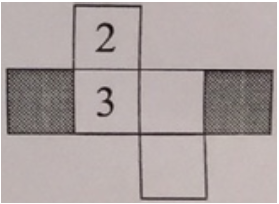
\includegraphics[scale=0.35]{177.png}}
\end{figure}
\end{center}
